\documentclass[./presentation_main.tex]{subfiles}
\begin{document}
\begin{frame}[c]{Magnetic Field Regions}
    \begin{columns}[T]
\column{0.5\linewidth}
\begin{itemize}
    \item<1-> Three regions
        \begin{itemize}[label=--]
            \item<2-> Solar Wind
            \item<3-> \textit{Magnetosheath}
            \item<4-> Magnetosphere
        \end{itemize}
\end{itemize}
\column{0.5\linewidth}
        \only<1>{\only<1>{\vphantom{\includesvg[width=\linewidth]{magnetic_regions_magnetosphere.svg}}}}
        \only<2>{
            \begin{figure}[H]
                \raggedleft
                \includesvg[width=\linewidth]{magnetic_regions_solar_wind.svg}
                \label{figsolarwind}
            \end{figure}
            %
        }
        \only<3>{
            \begin{figure}[H]
                \raggedleft
                \includesvg[width=\linewidth]{magnetic_regions_magnetosheath.svg}
                \label{figsolarwind}
            \end{figure}
            %
        }
        \only<4>{
            \begin{figure}[H]
                \raggedleft
                \includesvg[width=\linewidth]{magnetic_regions_magnetosphere.svg}
                \label{figsolarwind}
            \end{figure}
            %
        }
\end{columns}
\end{frame}
\begin{frame}[c]{Boundary Crossing}
\only<1>{
\begin{figure}[H]
    \centering
    \includesvg[width=0.7\linewidth]{messenger_orbit.svg}
    \label{figmessengerorbit}
\end{figure}
}
%
\only<2>{
\begin{figure}[H]
    \centering
    \includesvg[width=0.7\linewidth]{messenger_orbit_crossings.svg}
    \label{figboundarycrossing}
\end{figure}
}
\end{frame}
\begin{frame}[c]{Variability of Boundaries}
    \only<1>{
\begin{figure}[H]
    \centering
    \includesvg[width=0.7\linewidth]{messenger_orbit_variable_boundaries.svg}
    \label{figvariabilityboundary}
\end{figure}
%
    }
\only<2>{
\begin{figure}[H]
    \centering
    \includesvg[width=\linewidth]{messenger_orbit_multiple_crossings.svg}
    \label{figmultiplecrossings}
\end{figure}
%
}
\end{frame}
\begin{frame}[c]{Encounters}
\begin{figure}[H]
    \centering
    \includesvg[width=\linewidth]{messenger_orbit_encounters.svg}
    \label{figencounter}
\end{figure}
%
\end{frame}
\begin{frame}[c]{Regions, Crossings, \& Encounters on MAG Data}
    \only<1>{
        \begin{figure}[H]
            \centering
            \includesvg[width=0.8\linewidth]{./images/plots/mp_crossings.svg}
            \label{figmpcrossingsmag}
        \end{figure}
        %
    }
    \only<2>{
        \begin{figure}[H]
            \centering
            \includesvg[width=0.8\linewidth]{./images/plots/crossings_subplot.svg}
            \label{figbscrossingsmag}
        \end{figure}
        %
    }
\end{frame}
\begin{frame}[c]{Defining an Orbit}
    \only<2>{
\begin{figure}[H]
    \centering
    \includesvg[width=0.6\linewidth]{precession.svg}
    \label{figprecession}
\end{figure}
%
}
\only<3>{
    \vspace{-10pt}
    \begin{columns}[T]
        \column{0.5\linewidth}
        \begin{figure}[H]
            \centering
            \includesvg[width=\linewidth]{precession.svg}
            \label{figprecession}
        \end{figure}
        \column{0.5\linewidth}
        \begin{figure}[H]
            \centering
            \includesvg[width=\linewidth]{../plots_and_images/orbits_plot_with_peaks.svg}
            \captionsetup{font=scriptsize}
            \caption{Plot of radial distance from Mercury over a few days. The red crosses mark the periapsides, while the rest of the crosses mark the type of boundary crossing.}
            \label{figephemerisdata}
        \end{figure}
          
    \end{columns}
    %
}
\only<4>{
    \vspace{-10pt}
    \begin{figure}[H]
        \centering
        \includesvg[width=0.75\linewidth]{../plots_and_images/hollman_orbit_times.svg}
        \captionsetup{font=scriptsize}
        \caption{Lengths of orbits found from ephemeris data.}
        \label{figorbitlengths}
    \end{figure}
    %
}
\end{frame}
\begin{frame}[c]{Transition Orbits}
\begin{figure}[H]
    \centering
    \includesvg[width=\linewidth]{./images/plots/transitions_orbits.svg}
    \label{figtransitionorbits}
\end{figure}
%
\end{frame}
\begin{frame}[c]{MESSENGER Capture}
\begin{figure}[H]
    \centering
    \includesvg[width=0.65\linewidth]{./images/plots/orbit_capture.svg}
    \captionsetup{font=scriptsize}
    \caption{\scriptsize MESSENGER being captured by Mercury, first orbit start is $\sim$ 2011-03-18 00:00.}
    \label{figorbitcapture}
\end{figure}
%
\end{frame}
\begin{frame}[c]{Number of Crossings per Orbit}
\pause
\vspace{-10pt}
\begin{figure}[H]
    \centering
    \includesvg[width=0.7\linewidth]{crossings_per_orbit_hollman.svg}
    \captionsetup{font=scriptsize}
    \caption{Histogram of number of crossing per orbit using Hollman's 2025 list of crossings, determined with a region classifier machine learner algorithm.}
    \label{fighollmancrossings}
\end{figure}
%
\end{frame}
\begin{frame}[c]{Number of Crossing per Orbit}
\begin{figure}[H]
    \centering
    \includesvg[width=0.75\linewidth]{crossings_per_orbit_hollman_log.svg}
    \label{figloghollman}
\end{figure}
%
\end{frame}
\begin{frame}[c]{Hollman MESSENGER Region Classifier}
\begin{figure}[H]
    \centering
    \includesvg[width=0.35\linewidth]{./images/plots/hollman_model.svg}
    \caption{}
    \label{fighollmanmodel}
\end{figure}
%
\end{frame}
\begin{frame}[c]{Number of Each Crossing Type per Orbit}
\begin{figure}[H]
    \centering
    \includesvg[width=0.6\linewidth]{../plots_and_images/hollman_bs_mp_per_orbit.svg}
    \caption{\scriptsize Number of crossing of each type per orbit in the Hollman list.}
    \label{fignumberofcrossingtype}
\end{figure}
%
\end{frame}
\begin{frame}[c]{Extrema Analysis}
    \only<1>{
        \begin{figure}[H]
            \begin{subfigure}[H]{0.4\linewidth}
            \includesvg[width=\linewidth]{../plots_and_images/orbit_with_42_crossings.svg}
            \end{subfigure}
            \begin{subfigure}[H]{0.4\linewidth}
            \includesvg[width=\linewidth]{../plots_and_images/orbit_with_54_crossings.svg}
            \end{subfigure}
            %
            \label{figextrema}
        \end{figure}
        %
    }
\end{frame}
\begin{frame}[c]{Extrema MAG Data}
\only<1>{
\begin{figure}[H] 
\begin{subfigure}[H]{0.45\linewidth}
    \includesvg[width=\linewidth]{../plots_and_images/mag_with_42_crossings.svg}
\end{subfigure}
\begin{subfigure}[H]{0.45\linewidth}
    \includesvg[width=\linewidth]{../plots_and_images/mag_with_54_crossings.svg}
\end{subfigure}
%
\end{figure}
%
}
\only<2>{
\begin{figure}[H] 
\begin{subfigure}[H]{0.45\linewidth}
    \includesvg[width=\linewidth]{../plots_and_images/mag_with_42_crossings_zoom.svg}
\end{subfigure}
\begin{subfigure}[H]{0.45\linewidth}
    \includesvg[width=\linewidth]{../plots_and_images/mag_with_54_crossings_zoom.svg}
\end{subfigure}
%
\end{figure}
%

}
\end{frame}
\begin{frame}[c]{Orbit Plots}
    \only<1>{
        \begin{figure}[H]
            \centering
            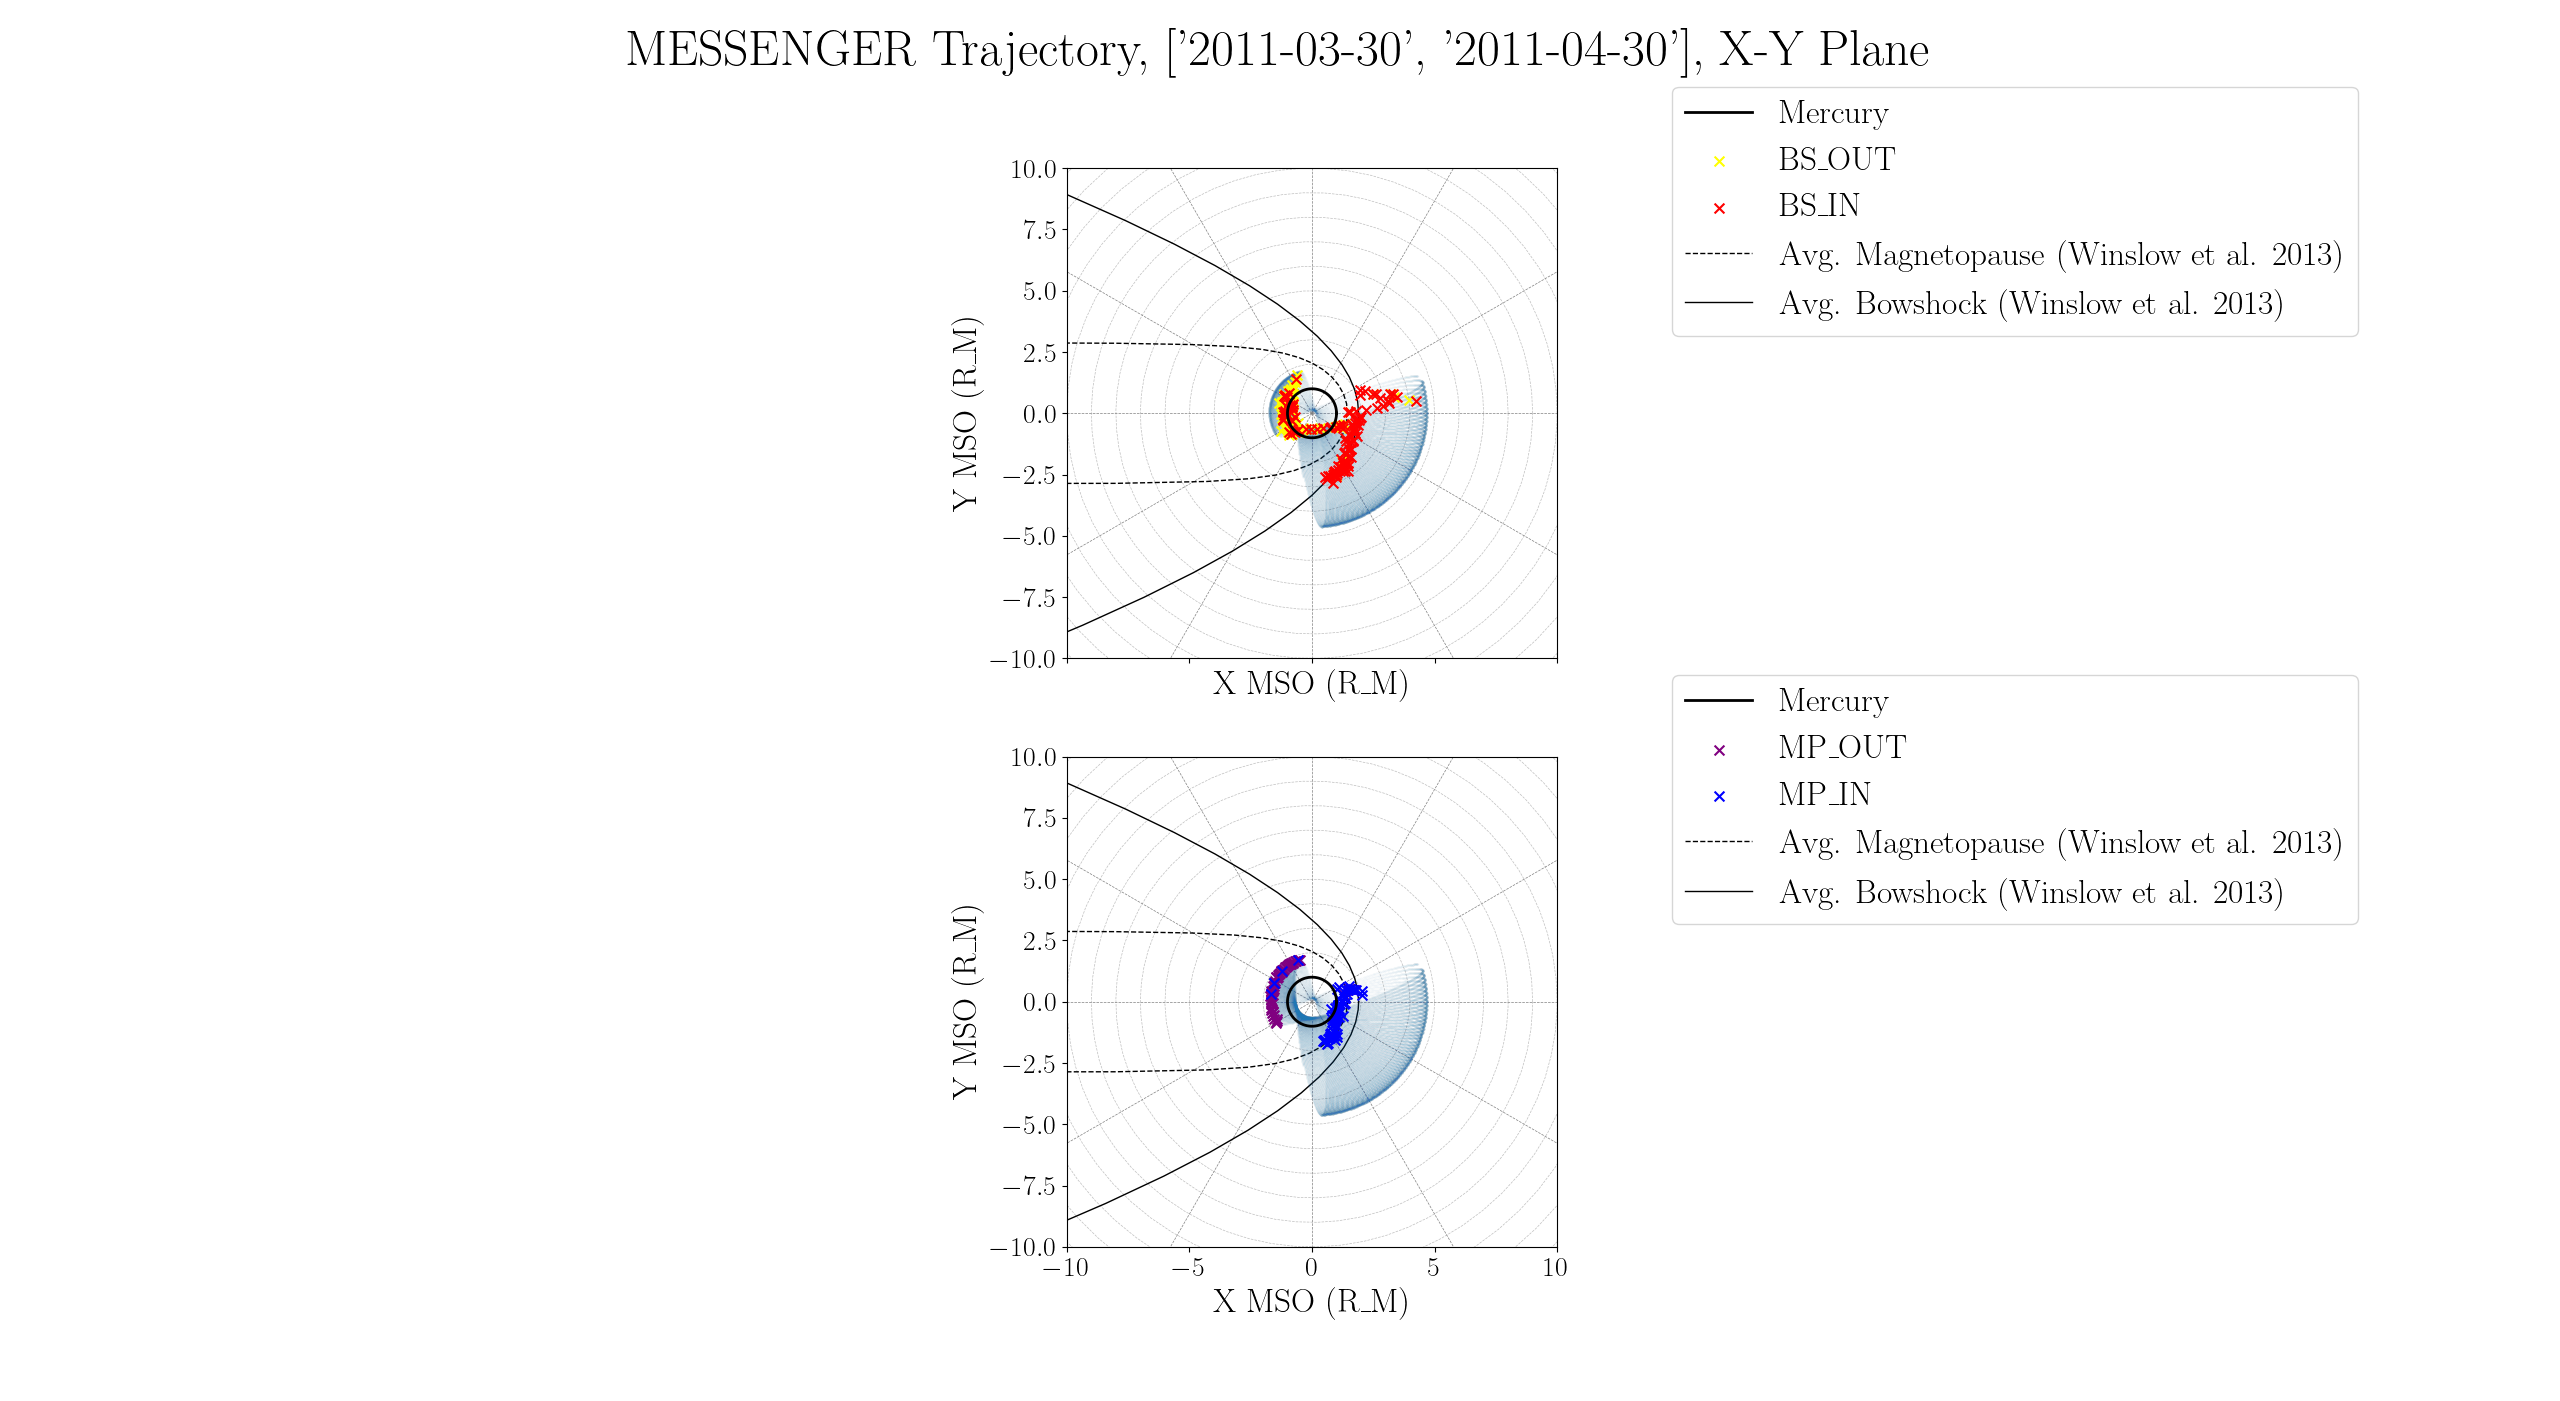
\includegraphics[width=\linewidth]{./images/plots/orbit_XY_crossings.png}
            \captionsetup{font=footnotesize}
        \end{figure}
        %
    }
    \only<2>{
        \begin{figure}[H]
            \centering
            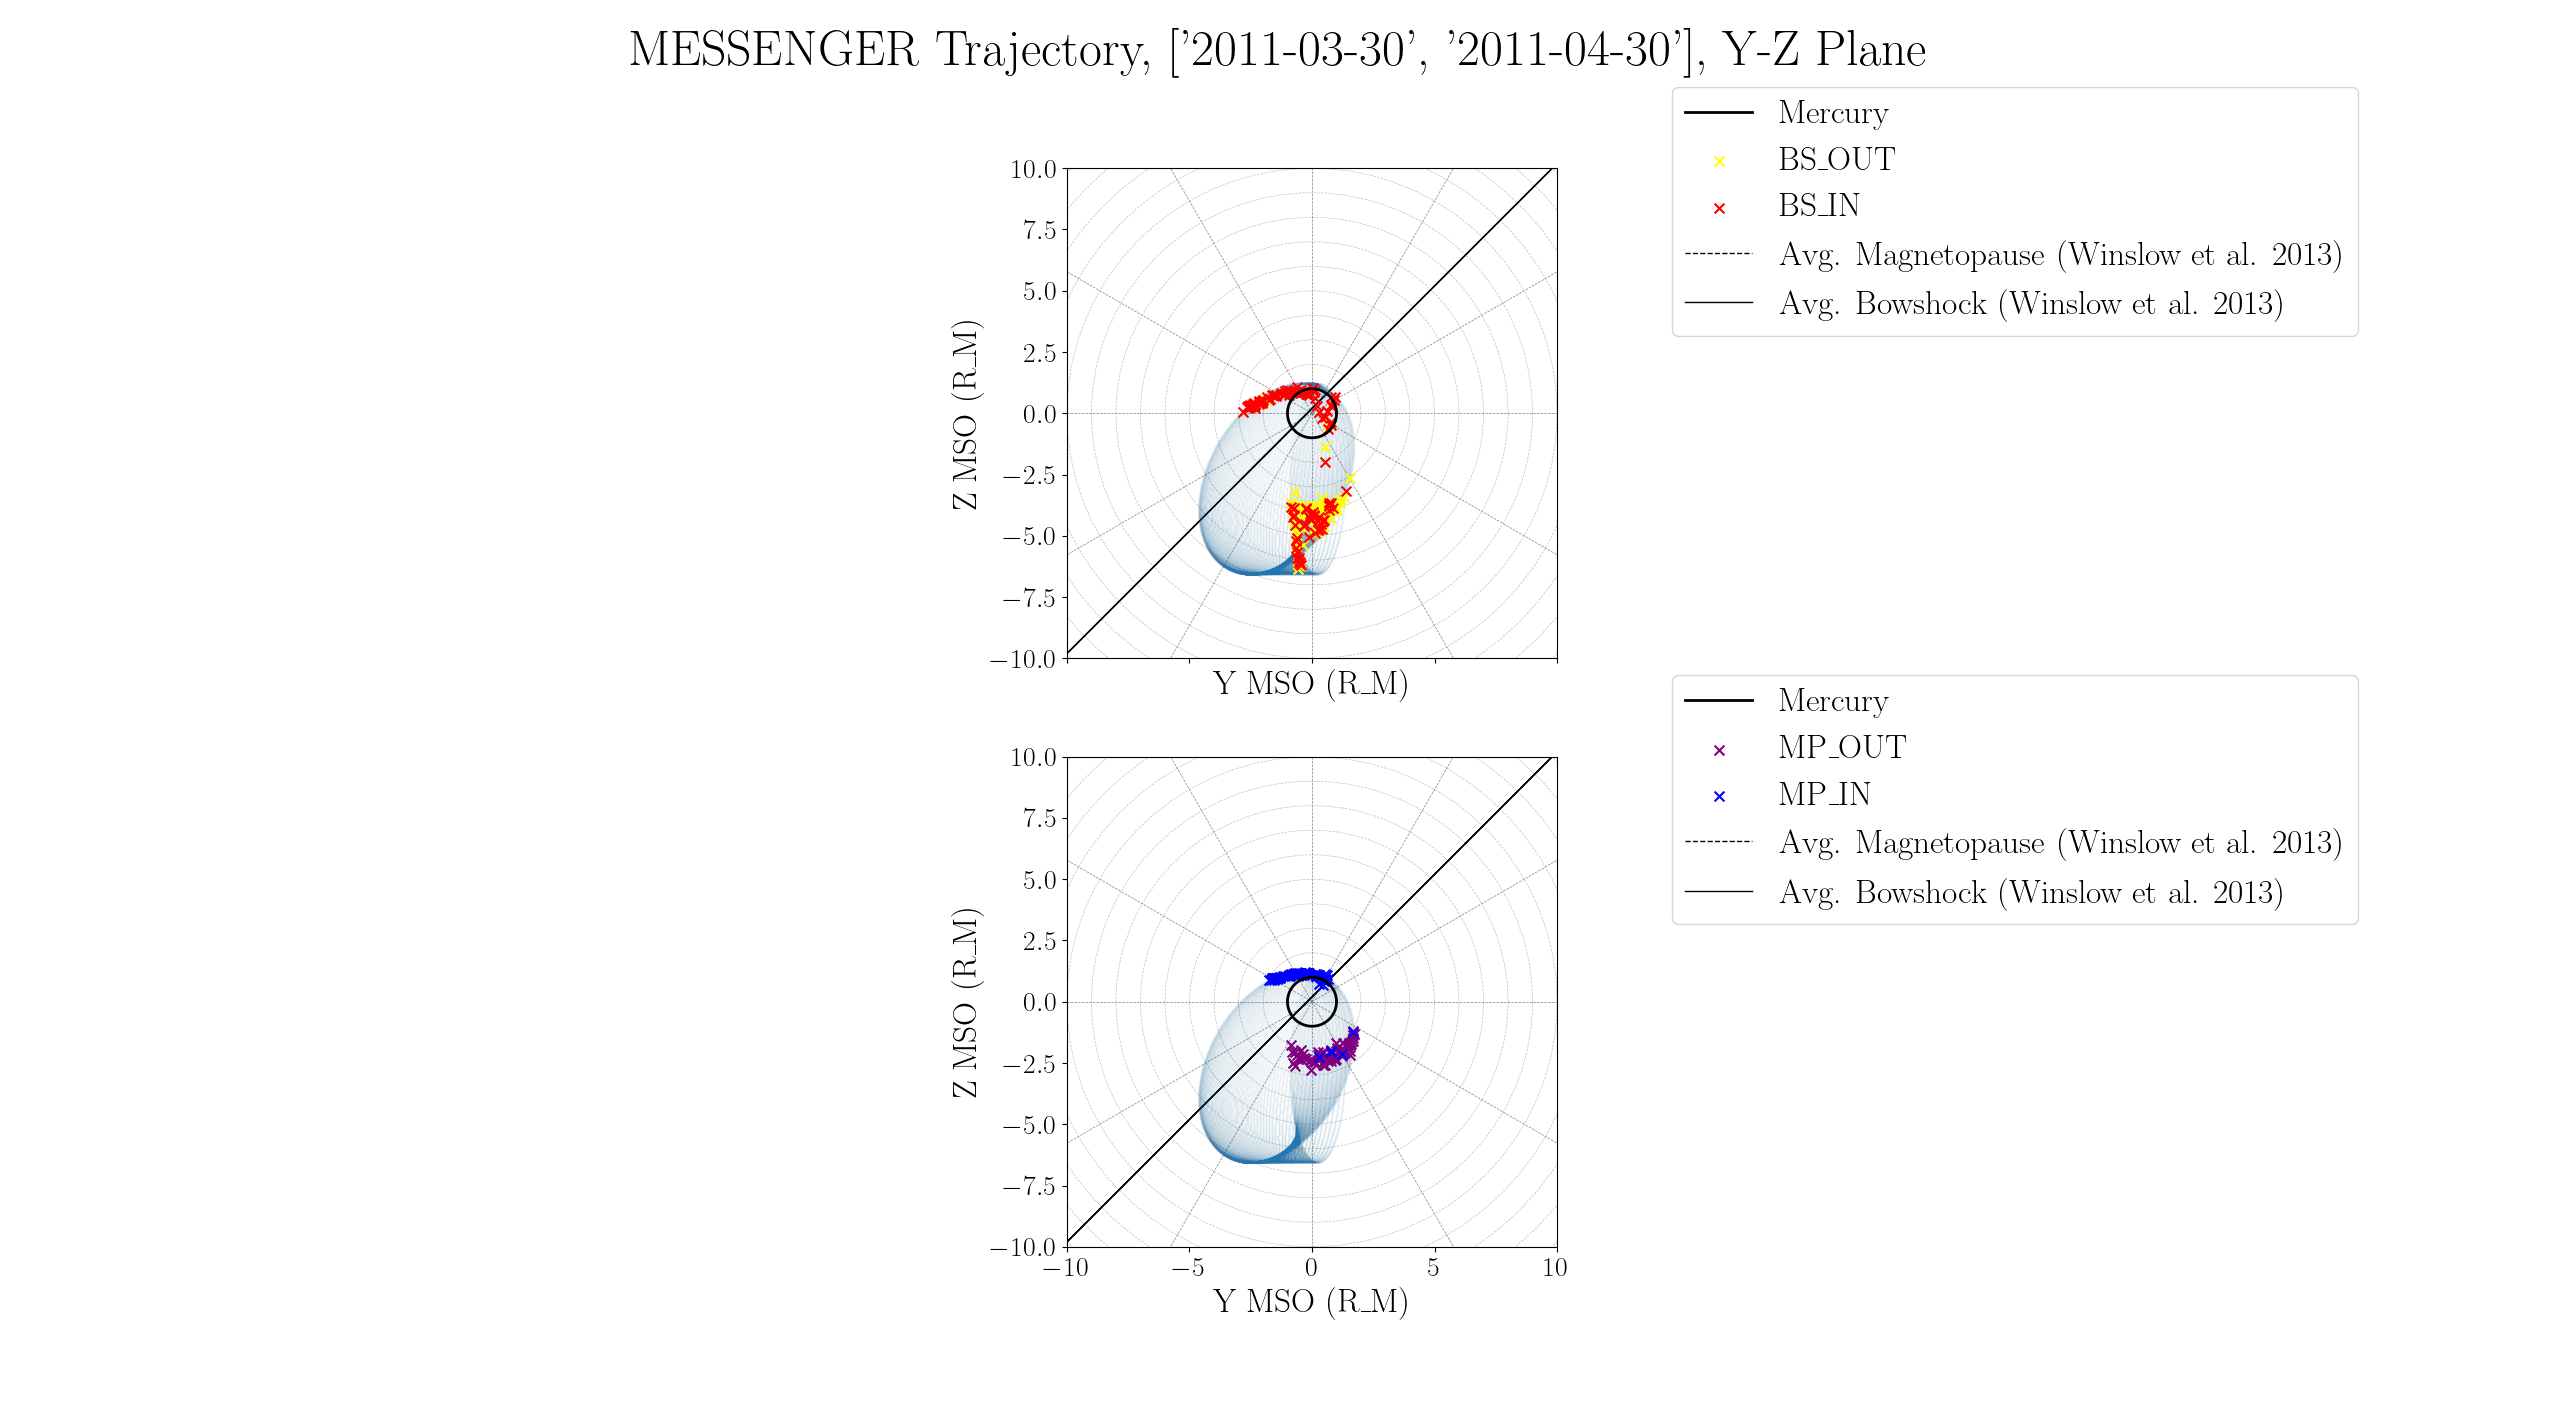
\includegraphics[width=\linewidth]{./images/plots/orbit_YZ_crossings.png}
            \captionsetup{font=footnotesize}
        \end{figure}
        %
    }
    \only<3>{
        \begin{figure}[H]
            \centering
            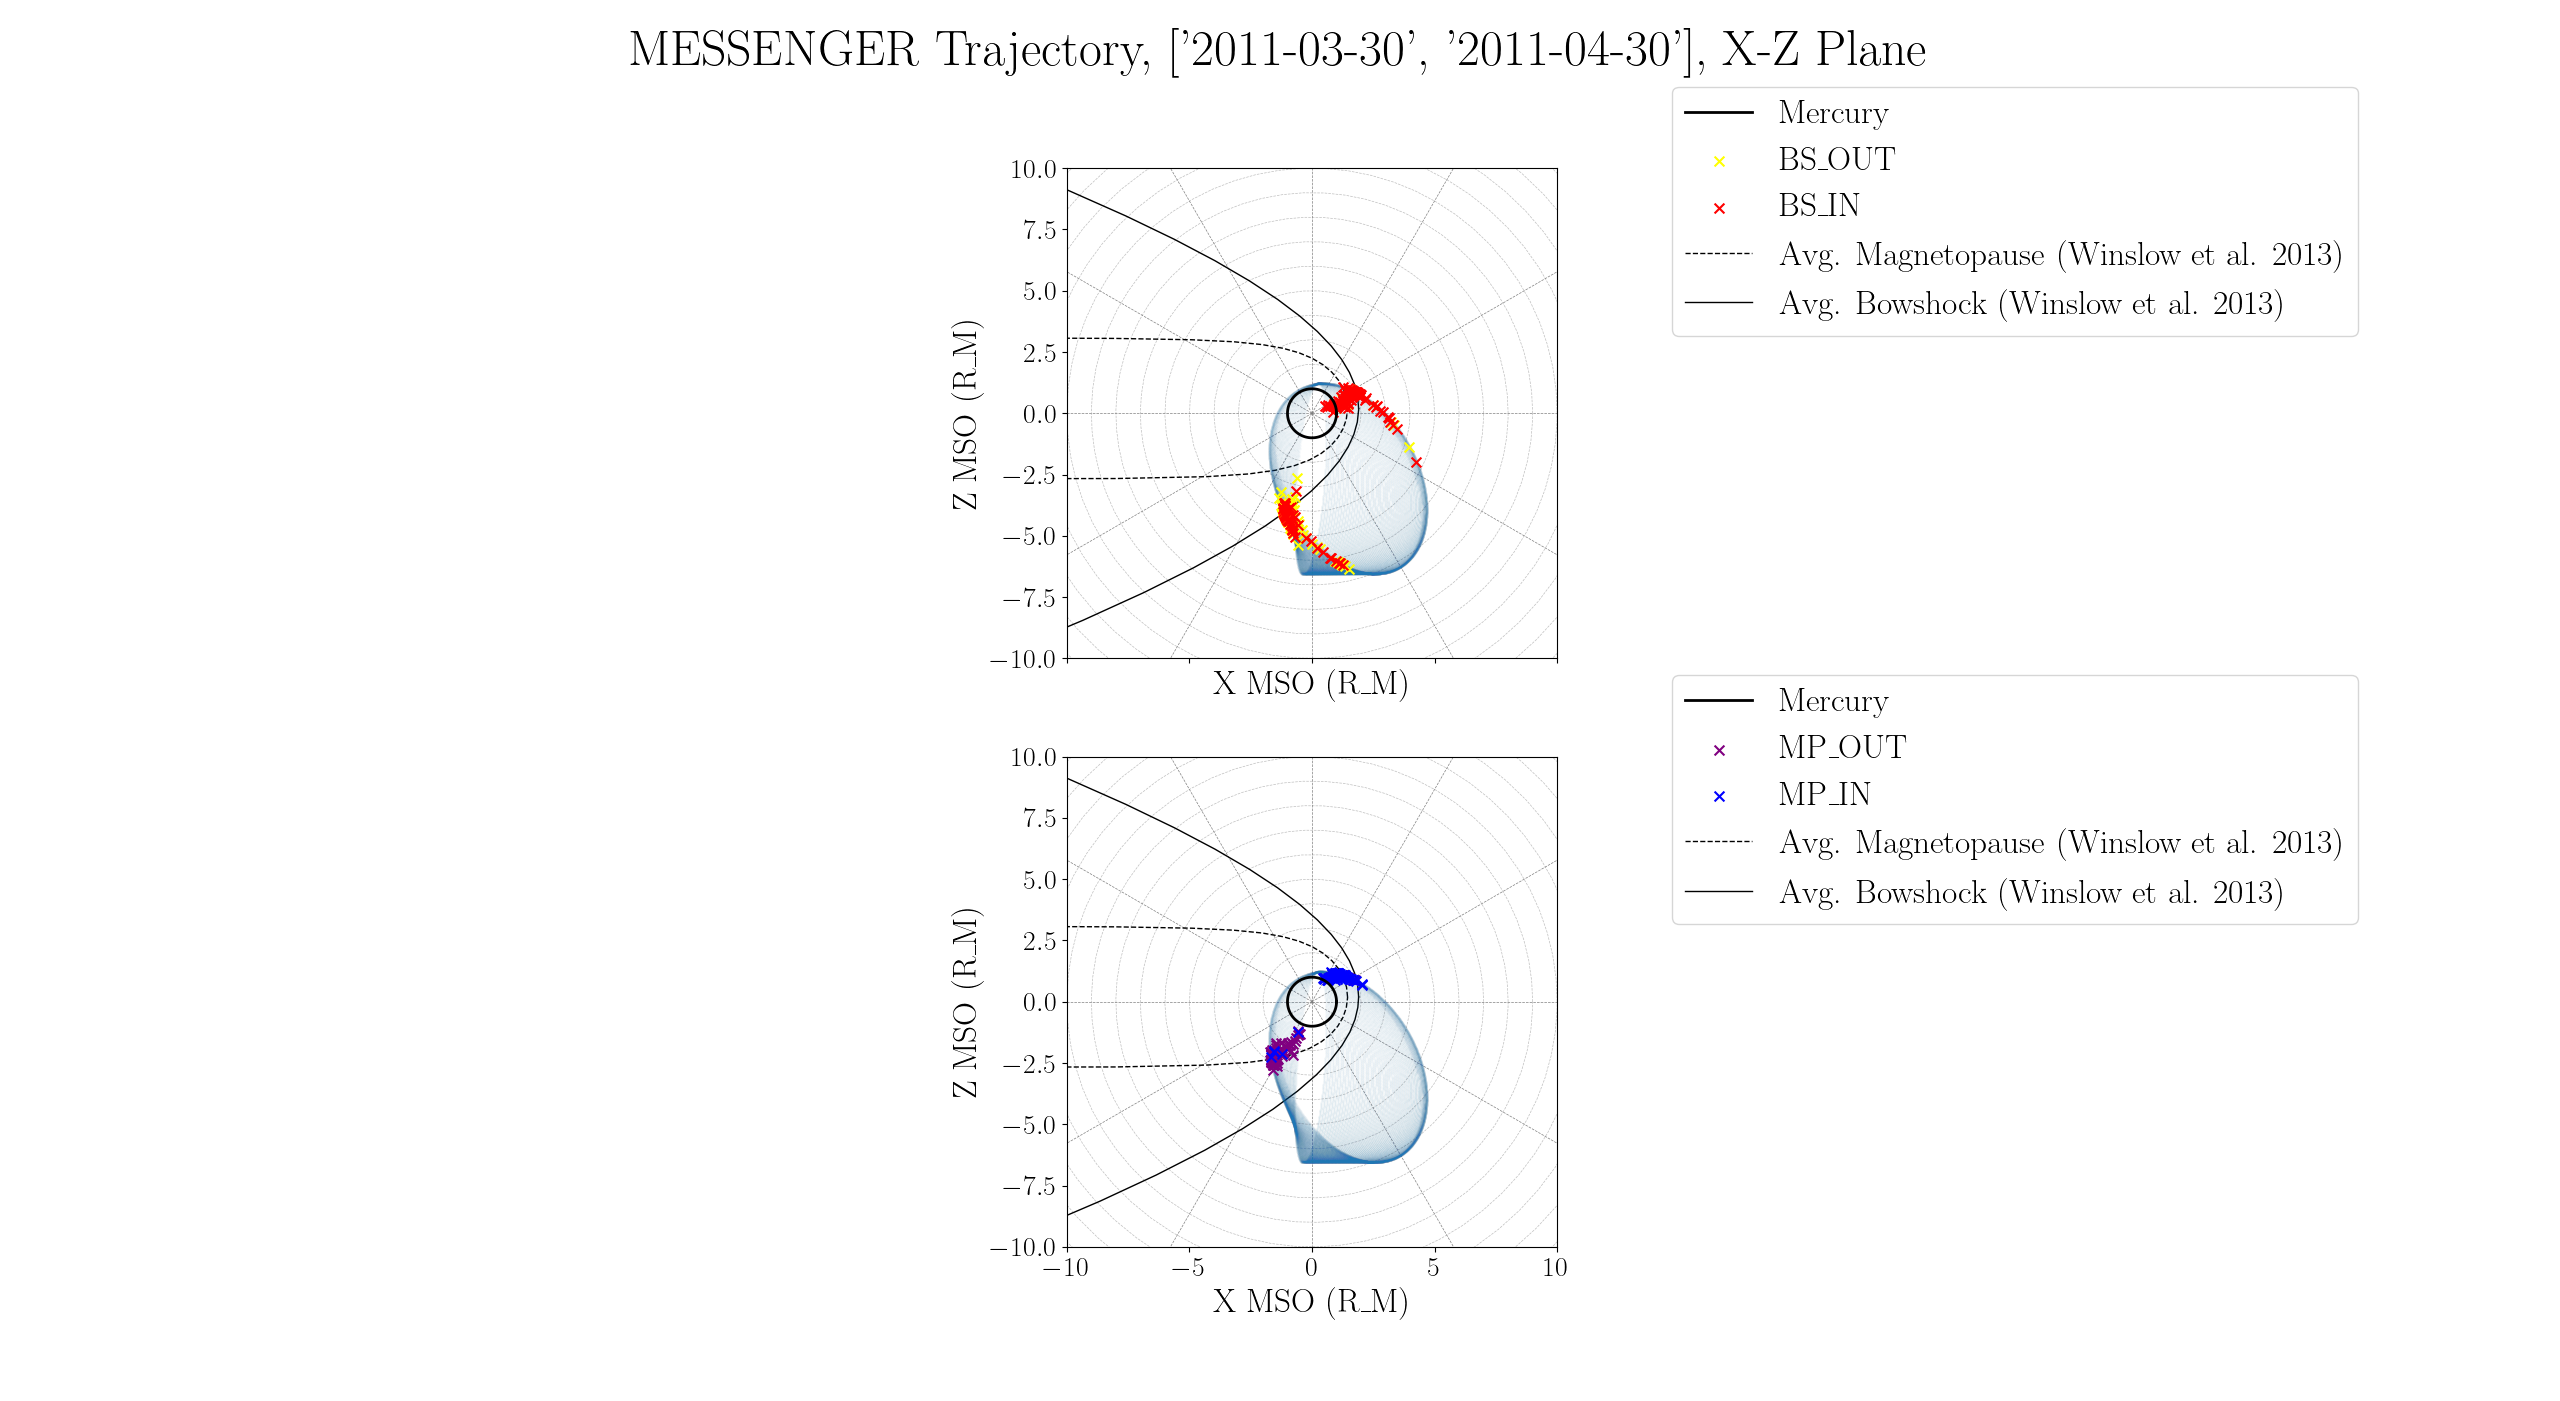
\includegraphics[width=\linewidth]{./images/plots/orbit_XZ_crossings.png}
            \captionsetup{font=scriptsize}
        \end{figure}
        %
    }
\end{frame}
\begin{frame}[c]{Time Between Crossings}
\begin{figure}[H]
    \centering
    \includesvg[width=0.7\linewidth]{../plots_and_images/hollman_crossings_dt.svg}
    \captionsetup{font=scriptsize}
    \caption{}
    \label{figdtbetweencrossings}
\end{figure}
%
\end{frame}
\begin{frame}[c]{Time Between Each Crossing Type}
\begin{figure}[H]
    \centering
    \includesvg[width=0.55\linewidth]{../plots_and_images/hollman_crossings_dt_bs_mp.svg}
    \captionsetup{font=scriptsize}
    \caption{}
    \label{figdtbetweencrossingsbsmp}
\end{figure}
%
\end{frame}
\begin{frame}[c]{Encounters}
\begin{figure}[H]
    \centering
    \includesvg[width=0.65\linewidth]{../plots_and_images/encounters_per_orbit.svg}
    \captionsetup{font=scriptsize}
    \caption{Number of orbits per encounter}
    \label{fig}
\end{figure}
%
\end{frame}
\begin{frame}[c]{Encounter Duration}
\begin{figure}[H]
    \centering
    \includesvg[width=0.7\linewidth]{../plots_and_images/Hollman_dt_encounters.svg}
    \caption{}
    \label{fighollmanencounterduration}
\end{figure}
%
\end{frame}
\begin{frame}[c]{Time Between Encounters}
    \only<1>{
\begin{figure}[H]
    \centering
    \includesvg[width=0.8\linewidth]{../plots_and_images/Hollman_dt_encounters_all.svg}
    \captionsetup{font=footnotesize}
    \caption{Time between encounters, defined from the Hollman 2025 list.}
    \label{fighollmandtencounters}
\end{figure}
%
    }
    \only<2>{
        \begin{figure}[H]
            \centering
            \includesvg[width=0.6\linewidth]{../plots_and_images/Hollman_dt_encounters_bs_mp.svg}
            \captionsetup{font=footnotesize}
            \caption{Time between BS encounters and MP encounters.}
            \label{fighollmandtencountersbsmp}
        \end{figure}
        %
    }
\end{frame}
\begin{frame}[c]{Comparison with Other Available Data Sets}
    \only<1>{
        \begin{figure}[H]
            \centering
            \includesvg[width=0.8\linewidth]{../plots_and_images/Sun et al._dt_encounters_all.svg}
            \captionsetup{font=footnotesize}
            \caption{}
            \label{figsunencounters}
        \end{figure}
        %
    }
    \only<2>{
        \begin{figure}[H]
            \centering
            \includesvg[width=0.8\linewidth]{../plots_and_images/Philpott et al._dt_encounters_all.svg}
            \captionsetup{font=footnotesize}
            \caption{}
            \label{figsunencounters}
        \end{figure}
        %
    }
\end{frame}
\begin{frame}[c]{Sun \& Philpott List MP \& BS Crossings}
\begin{figure}[H] 
\begin{subfigure}[H]{0.45\linewidth}
    \includesvg[width=\linewidth]{../plots_and_images/Sun et al._dt_encounters_bs_mp.svg}
\end{subfigure}
\begin{subfigure}[H]{0.45\linewidth}
    \includesvg[width=\linewidth]{../plots_and_images/Philpott et al._dt_encounters_bs_mp.svg}
\end{subfigure}
%
\end{figure}
%
\end{frame}
\begin{frame}[c]{Data Comparison (Cumulative Distribution Function)}
    \only<1>{
\begin{figure}[H] 
    \includesvg[width=0.6\linewidth]{../plots_and_images/cdf_sun_phil.svg}
\end{figure}
%
    }
    \only<2>{
        \begin{figure}[H] 
        \begin{subfigure}[H]{0.45\linewidth}
            \includesvg[width=\linewidth]{../plots_and_images/cdf_hollman_sun.svg}
        \end{subfigure}
        \begin{subfigure}[H]{0.45\linewidth}
            \includesvg[width=\linewidth]{../plots_and_images/cdf_hollman_phil.svg}
        \end{subfigure}
        %
        \end{figure}
        %
    }
\end{frame}
\end{document}
